\documentclass[10pt,a4paper]{article}
\usepackage[utf8]{inputenc}
\usepackage[german]{babel}
\usepackage{amsmath}
\usepackage{amsfonts}
\usepackage{amssymb}
\usepackage{setspace}
\usepackage{graphicx} %Um Bilder anzeigen zu können
\usepackage[top=1in, bottom=1.5in, left=1in, right=1in]{geometry}

\title{\Huge Pflichtenheft\\[1cm] {\bfseries Praxis der Softwareentwicklung}\\[2cm] Entwicklung einer Software zur Berechnung der Mandatsverteilung im Deutschen Bundestag\\[1cm]Gruppe 1}
\author{Philipp Löwer, Anton Mehlmann, Manuel Olk, Enes Ördek, \\Simon Schürg, Nick Vlasoff}
\date{}

\begin{document}
\maketitle
\thispagestyle{empty}

\begin{figure}[h]

\centering
		
		
\includegraphics[scale=0.6]{KIT-Logo.png}\\
		\Huge WS 2013 / 14
\end{figure}

\newpage
\begin{onehalfspace}
\tableofcontents
\end{onehalfspace}
\newpage 

\section{Produktübersicht}
Das Produkt soll allen Personen, auch ohne spezifisches Vorwissen, die sich mit der Deutschen Bundestagswahl beschäftigen, als Unterstützung dienen.\newline
Dafür ist die Aufbereitung von Wahlergebnissen gemäß der gesetzlichen Bestimmungen und deren exakte und übersichtliche Darstellung, z.B. der endgültigen Sitzverteilung im Deutschen Bundestag, essentiell.
Da das aktuelle Wahlsystem sehr komplex ist, besteht eine weitere Aufgabe des Programms darin, das Zustandekommen von Direktmandaten, Überhangmandaten, Ausgleichsmandaten usw. dem Anwender verständlich zu erklären.
Darunter fallen auch paradox erscheinende Vorkommnisse, wie das negative Stimmgewicht, die durch das Programm gefunden und erklärt werden sollen. \newline
Des Weiteren ermöglicht die Anwendung mit beliebigen Wahldaten zu experimentieren und die daraus resultierenden Veränderungen anzuzeigen. Dadurch lässt es sich auch gut für Demonstrationen (z.B. für das Aufzeigen von Rundungsfehlern bei der Sitzberechnung) nutzen.


\subsection{Lizenz}
Es gibt bereits kommerzielle Programme, die dem Produkt ähneln. Diese sind aber nicht frei verfügbar und weisen meistens gerade in Bezug auf die Nutzerfreundlichkeit für Laien erhebliche Mängel auf. Genau dort wird nun Abhilfe geschafft.\newline
Der Quellcode wird der Öffentlichkeit frei zur Verfügung gestellt, um Interessenten die Bundestagswahl und ihre Besonderheiten kostenlos und nachvollziehbar näher zu bringen. Es wird die GPL V3 Lizenz verwendet, damit das Projekt beliebig erweitert bzw. modifiziert werden kann und trotzdem immer noch als freie Software gilt.



\section{Zielbestimmung}
\subsection{Musskriterien}
\begin{itemize}
\item Auswertung von Wahlergebnissen nach gesetzlicher Bestimmung
\begin{itemize}
\item Berechnen der Direkt-, Überhang- und Ausgleichsmandate
\item Berechnen der restlichen Sitzverteilung im Deutschen Bundestag anhand der Zweitstimmen
\end{itemize}
\item Anzeigen und Interaktion mit Wahlausgängen anhand einer grafischen Benutzeroberfläche
\item Direkte Gegenüberstellung verschiedener Wahlausgänge (z.B. Wahlausgang 2013 - Wahlausgang 2009)
\item Importmöglichkeit von Wahlergebnissen (.csv)
\item Manuelle Änderung von importierten Wahlergebnissen (z.B. Zweitstimmen für eine Partei erhöhen)
\end{itemize}

\subsection{Sollkriterien}
\begin{itemize}
\item Auffinden von Wahlausgängen zu paradoxen Vorkommnissen (z.B. negatives Stimmgewicht)
\item Kartografische Darstellung der Bundesländer
\end{itemize}

\subsection{Kannkriterien}
\begin{itemize}
\item Hilfe (Benutzerhandbuch)
\item Anzeigen von Koalitionsmöglichkeiten
\end{itemize}


\subsection{Abgrenzungskriterien}
\begin{itemize}
\item Keine mobile Anwendung oder Web- Applikation
\item Keine Übersetzung in andere Sprachen
\item Keine namentliche Nennung von Abgeordneten
\end{itemize}


\section{Produkteinsatz}
\subsection{Anwendungsbereiche}
\begin{itemize}
\item Kann genutzt werden, ...
\begin{itemize}
\item um Wahlausgänge zu simulieren
\item um komplexes Wahlsystem nachzuvollziehen 
\item um bestimmte Sachverhalte (z.B. negatives Stimmrecht, Benachteiligung kleiner Parteien) darzustellen 
\end{itemize} 
\end{itemize}


\subsection{Zielgruppen}
\begin{itemize}
\item Politisch Interessierte
\item Medien (z.B. Internetseiten, regionale Zeitungen)
\end{itemize}


\subsection{Betriebsbedingungen}
\begin{itemize}
\item Die Verbindung zum Internet ist optional
\end{itemize}


\section{Produktumgebung}
\subsection{Software}
\begin{itemize}
\item Java Runtime Environment SE 1.7 oder neuer.
\item Betriebssystem z.B. Windows, Linux, Mac OS
\end{itemize}


\subsection{Hardware}
Das Programm ist für den Einsatz auf PCs oder Laptops geeignet.
\subparagraph{Mindestanforderungen:}
\begin{itemize}
\item 128 MB Arbeitsspeicher
\item 100 MB freien Festplattenspeicher
\item 500-MHz-Prozessor
\item Farbdisplay/ Bildschirmauflösung: 1024x768
\end{itemize}

\subparagraph{Empfohlen:}
\begin{itemize}
\item 512 MB Arbeitsspeicher
\item 100 MB freien Festplattenspeicher
\item 1-GHz-Prozessor
\item Farbdisplay/ Bildschirmauflösung: 1024x768
\end{itemize}


\subsection{Orgware}
\begin{itemize}
\item Keine weiteren Rahmenbedingungen notwendig
\end{itemize}


\subsection{Schnittstellen}
\begin{itemize}
\item Importieren/Exportieren von Wahldaten (.csv)
\end{itemize}


\section{Funktionale Anforderungen}
Funktionale Anforderungen werden durch eine vierstellige Nummer gekennzeichnet. Die erste Nummer kennzeichnet den folgenden Bereich:
\begin{enumerate}
	\item GUI
	\item Schnittstellen
	\item Datenhaltung
\end{enumerate}
Die restlichen Nummern dienen zur Durchnummerierung.

\subsection{GUI}
\begin{description}
	\item \textbf{/F10005/} Programmstart \hfill \\
	Es erscheint das Programmfenster (/F10050/), in dem die Wahlergebnisse 2013 voreingetragen wurden. Die dazugehörige Sitzverteilung wird automatisch berechnet.
	\item \textbf{/F10010/} Menü \hfill \\
	Im Menü sind folgende Punkte gelistet:
		
	\begin{itemize}
		\item Datei
		\begin{itemize}
			\item Neuer Tab /F10015/
			\item Tab schließen /F10020/
			\item Laden /F20010/
			\item Speichern /F20020/
			\item Beenden /F10025/
		\end{itemize}
		\item Bearbeiten
		\begin{itemize}
			\item Rückgängig /F10030/
			\item Wiederherstellen /F10035/
		\end{itemize}
		\item Extras
		\begin{itemize}
			\item Vergleichen /F10075/
			\item Wahldaten generieren /F30030/
		\end{itemize}
		\item Hilfe
		\begin{itemize}
			\item Benutzerhandbuch /F10040/
			\item Über /F10045/
		\end{itemize}	
	\end{itemize}
	\item \textbf{/F10015/} Neuer Tab \hfill \\
	Beim Anklicken wird ein neuer Tab generiert, in dem eine neue Bundestagswahl (/PD01/) geladen werden kann. Diese Dateiauswahl korrespondiert zu dem '+'-Button in der Tab-Leiste.
	\item \textbf{/F10020/} Tab schließen \hfill \\
	Beim Anklicken wird der aktuelle Tab geschlossen. Wurden Änderung an den Daten (/PD01/) vorgenommen, wird vor dem Schließen des Tabs dem Benutzer die Möglichkeit gegeben die Daten zu speichern, zu verwerfen oder das Schließen abzubrechen.
	\item \textbf{/F10025/} Beenden \hfill \\
	Beendet das gesamte Programm. Wurden Änderung an den Daten (/PD01/) vorgenommen, wird vor dem Schließen des Tabs dem Benutzer die Möglichkeit gegeben die Daten zu speichern, zu verwerfen oder das Schließen abzubrechen.
	\item \textbf{/F10030/} Rückgängig machen \hfill \\
	Wurde eine Stimmzahl, ob in einem Wahlkreis oder in einem ganzen Bundesland, verändert, kann die Änderung bis zu fünf Mal widerrufen werden.
	\item \textbf{/F10035/} Wiederherstellen \hfill \\
	Falls Änderungen rückgängig gemacht wurden (/F10030/), können diese wieder hergestellt werden.
	\item \textbf{/F10040/} Benutzerhandbuch \hfill \\
	Enthält Informationen, die zur Benutzung des Programms hilfreich sind.
	\item \textbf{/F10045/} Über \hfill \\
	Enthält allgemeine Informationen über diese Software.
	\item \textbf{/F10050/} Programmfenster \hfill \\
	Das Programmfenster wird in drei Bereiche aufgeteilt.
	\begin{itemize}
		\item Tabellenfenster /F10060/
		\item Diagrammfenster /F10065/
		\item Kartenfenster /F10070/
	\end{itemize}
	Es gibt hierbei drei verschiedene Ansichten.
	\begin{itemize}
		\item Bundesansicht /F10080/
		\item Landesansicht /F10085/
		\item Wahlkreisansicht /F10090/
	\end{itemize}
	\item \textbf{/F10060/} Tabellenfenster \hfill \\
	Im Tabellenfenster werden Details zu allen, an der Bundestagswahl teilnehmenden, Parteien angezeigt.
	Es gibt die Spalten Partei, Erst- und Zweitstimmen, Direkt-, Überhang- und Ausgleichsmandate, die in jeder Ansicht variieren. \hfill \\
	\item \textbf{/F10065/} Diagrammfenster \hfill \\
	Im Diagrammfenster werden Details, der aktuellen Auswahl entsprechend, angezeigt. Befindet man sich in der Bundesansicht (/F10080/) wird die Sitzplatzverteilung (/F10091/) für alle in den Bundestag einziehenden Parteien angezeigt. Wurde ein bestimmtes Bundesland vom Benutzer gewählt, zeigt das Diagramm die prozentuale Anzahl der Zweitstimmen, die die einzelnen Parteien bekommen haben. Nachdem ein Wahlkreis des Bundeslandes angeklickt wurde (/F10090/), sieht man die Erststimmen aller Wahlkreiskandidaten pro Partei. \hfill \\
	\item \textbf{/F10070/} Kartenfenster \hfill \\
	Im Kartenfenster wird, sofern möglich (/F30010/ Überprüfung der Ländernamen), eine kartografische Darstellung von Deutschland angezeigt oder die einzelnen Bundesländer aufgelistet, zwischen beiden kann mit Klick auf Reiter gewechselt werden. In der Karte werden diese nach der Farbe der Partei, die in diesem Bundesland die meisten Zweitstimmen erhielt, eingefärbt. Der Klick auf ein Bundesland öffnet eine Liste aller zugehörigen Wahlkreise, man gelangt zur Landesansicht (/F10085/). Zurückkehren kann man, indem man in der Liste auf das geöffnete Bundesland klickt oder in der Kartenansicht den Zurück-Button (/F10076) betätigt. Wählt man in der Landesansicht (/F10085/) einen Wahlkreis gelangt man in die Wahlkreisansicht (/F10090/). \hfill \\
	\item \textbf{/F10075/} Vergleichsfenster \hfill \\
	In diesem Fenster soll es möglich sein den Ausgang der Bundestagswahl des aktuellen Tabs mit einer anderen geladenen Bundestagswahl zu vergleichen. Ist keine andere Wahl gerade geöffnet, wird dem Benutzer erst empfohlen eine weitere Datei (/PD01/) in einen neuen Tab zu laden. \hfill \\
	\item \textbf{/F10076/} Zurück Button\hfill \\
	Man gelangt von der Wahlkreisansicht zurück in die Landesansicht und von der Landesansicht in die Bundesansicht. \hfill \\
	\item \textbf{/F10080/} Bundesansicht \hfill \\
	In dieser Ansicht wird ganz Deutschland betrachtet. Im Tabellenfenster (/F10060/) sieht man die Spalten Partei, Zweitstimmen, Direkt-, Überhangs- und Ausgleichsmandate. Im Diagrammfenster (/F10065/) sieht man ein Diagramm über die Sitzplatzverteilung im deutschen Bundestag. Im Kartenfenster (/F10070/) sieht man die gefärbte Deutschlandkarte oder eine Liste aller existierender Bundesländer. \hfill \\
	\item \textbf{/F10085/} Landesansicht \hfill \\
	In dieser Ansicht wird ein ausgewähltes Bundesland betrachtet. Im Tabellenfenster (/F10060/) gibt es die Spalten Partei, Zweitstimmen und Direktmandate. Im Diagrammfenster (/F10065/) sieht man ein Diagramm über die prozentuale Zweitstimmenanzahl der einzelnen Parteien. Im Kartenfenster (/F10070) sieht man eine Liste aller Wahlkreise des Bundeslandes. \hfill \\
	\item \textbf{/F10090/} Wahlkreisansicht \hfill \\
	In dieser Ansicht wird ein Wahlkreis des gewählten Bundeslandes betrachtet. Im Tabellenfenster /(/F10060/) gibt es die  Spalten Partei, Erst- und Zweitstimmen und eine Spalte, die anzeigt ob die jeweilige Partei ein Direktmandat erhält. Im Diagrammfenster (/F10065/) sieht man ein Diagramm über die prozentuale Erststimmenanzahl der einzelnen Wahlkreiskandidaten. Im Kartenfenster (/F10070/) wird der ausgewählte Wahlkreis markiert. \hfill \\
	\item \textbf{/F10091/} Sitzverteilung \hfill \\
	Die Sitzverteilung wird dargestellt mit einem Kuchendiagramm. Daneben kann man sich auch anzeigen lassen, wie jeder einzelne Sitz entstanden ist. Dies wird tabellarisch in einem neuen Fenster angezeigt. \hfill \\
	\item \textbf{/F10092/} Sortierung des Tabellenfensters \hfill \\
	Die Sortierung des Tabellenfensters kann mithilfe eines Klicks auf die Spaltenüberschriften geändert werden. \hfill \\
\end{description}

\subsection{Schnittstellen}
\begin{description}
	\item \textbf{/F20010/} Laden \hfill \\
	Es können Wahlergebnisse in Form von .csv-Dateien importiert werden. Das Format dieser Dateien muss dem der bereitgestellten .csv-Datei zur Wahl 2013 der Bundeswahlleiter-Webseite entsprechen.
	\item \textbf{/F20020/} Speichern \hfill \\
	Es besteht die Möglichkeit, Wahlergebnisse im vorher spezifizierten Format (/F20010/) als .csv-Datei zu exportieren.
\end{description}

\subsection{Datenhaltung und Verarbeitung}
\begin{description}
	\item \textbf{/F30010/} Überprüfen der Ländernamen \hfill \\
	Überprüft, ob die eingegebenen Ländernamen mit den vorgegebenen Bundesländern übereinstimmen (/PD04/). Falls alle Ländernamen gefunden werden, wird die kartografische Darstellung (/F10070/) aktiviert. Andernfalls kann die kartografische Darstellung nicht angezeigt werden, es wird nur die tabellarische Ansicht angezeigt.
	\item \textbf{/F30020/} Überprüfen der Stimmen\hfill \\
	Überprüft, ob mit den eingegebenen/importierten Stimmdaten eine gültige Sitzverteilung berechnet werden kann.		
	\item \textbf{/F30030/} Generierung von Wahldaten \hfill \\
	Es können Wahldaten mit gewünschten paradoxen Vorkommnissen generiert werden.
	\item \textbf{/F30040/} Manuelles Ändern einzelner Stimmzahlen \hfill \\
	Der Benutzer kann in dem Tabellenfenster (/F10060/) die Zahlen der aktuellen Wahlsimulation manuell anpassen.
	Diese haben sofortigen Einfluss auf Karten- (/F10060/) und Diagrammfenster (/F10065/).
	\item \textbf{/F30050/} Paradoxe Wahlausgänge \hfill \\
	Die aktuell geladenen Wahlausgänge (/PD01/) werden auf paradoxe Eigenschaften überprüft. Bei einem Auftreten wird ein Hinweis ausgegeben.
	\item \textbf{/F30060/} Auswerten der Wahlergebnisse \hfill \\
	Nachdem die Wahlergebnisse (/PD01/) entweder geladen oder verändert wurden (/F30070/), werden sie ausgewertet, d.h. die Sitzverteilung wird berechnet (/F30065/) und alle Bereiche werden angepasst.
	\item \textbf{/F30065/} Berechnung der Sitzverteilung \hfill \\
	Die Sitzverteilung des Bundestages wird anhand der Stimmen und den daraus resultierenden Direktmandaten, Überhangmandaten, Ausgleichsmandaten und den Abgeordneten die über die Landeslisten in den Bundestag einziehen berechnet. Anhand der Erststimmen werden zunächst die Direktmandate der jeweiligen Wahlkreise bestimmt (299 Direktmandate). Die verbleibende Sitzerteilung des Bundestages wird anhand der Zweitstimmen, die die jeweiligen Parteien erhielten, errechnet. Dadurch entstehen Überhang- und Ausgleichsmandate.
	\item \textbf{/F30070/} Verändern der Wahlergebnisse \hfill \\
	In dem Tabellenfenster (/F10060/) können Stimmzahlen einzelner Wahlkreise verändert werden.
	\item \textbf{/F30080/} Färben der Bundesländer \hfill \\
	Wurden Bundeslandnamen (/F30010/) und Stimmen (/F30020/) überprüft, werden die einzelnen Bundesländer mit der Farbe der Partei eingefärbt, die die meisten Zweitstimmen in diesem Bundesland erhalten hat.
	
\end{description}

\section{Produktdaten}
\begin{description}
	\item[\textbf{/PD01/}] Wahlergebnis
	\begin{itemize}
		\item Name der Wahl
		\item Kommentar (Quelle)
		\item Wahlkreis/Bundesland mit Stimmen je Partei
		\item Anzahl der Wahlberechtigten
		\item Wahlergebnisse 2009 und 2013
		\item Anzahl der (Erst- und Zweit-)Stimmen je Wahlkreis/Bundesland und Partei
	\end{itemize}
	
	\item[\textbf{/PD02/}] Parteien
	\begin{itemize}
		\item Farbe
		\item Vollständiger Name
		\item Kürzel
	\end{itemize}
	
	\item[\textbf{/PD03/}] Bundesland
	\begin{itemize}
		\item Wappen		
		\item Vollständiger Name
		\item Kürzel
	\end{itemize}
	
	\item[\textbf{/PD04/}] Handbuch
	\begin{itemize}
		\item Informationen zum Programm (About)
		\begin{itemize}
			\item Autoren
			\item Webseite
		\end{itemize}
		\item Informationen zum Wahlsystem
	\end{itemize}
\end{description}

\section{Produktleistungen}
\begin{itemize}
	\item Zeit \hfill \\
	Das Programm muss fähig sein, Operationen auf Daten der letzten zwei Bundestagswahlen, in angemessener Zeit durchzuführen. Entscheidend sind hierbei die Anzahl der Parteien und die Anzahl der Wahlkreise.
	\\ Wir nehmen daher folgende Bedingungen an:
	\begin{itemize}
		\item etwa 30 Parteien
		\item etwa 300 Wahlkreise
		\item maximal 200.000.000 abgegebene Stimmen
	\end{itemize}
	Folgende Zeiten werden benötigt:
	\begin{itemize}
		\item Starten des Programms: unter 10 Sekunden
		\item Laden eines Zustandes: unter 10 Sekunden
		\item Berechnung der Sitzverteilung: unter 10 Sekunden
		\item Speichern eines Zustandes: unter 10 Sekunden
		\item Exportieren/Importieren von Daten: unter 10 Sekunden
		\item Beenden des Programms: unter 3 Sekunden
	\end{itemize}
	\item Genauigkeit \hfill \\
	Die Genauigkeit des Algorithmus zur Sitzberechnung muss dem Wahlgesetz entsprechen und exakte Ergebnisse liefern.
\end{itemize}


\section{Nicht-funktionale Anforderungen}
\subsection{Allgemeine Anforderungen}
Die Sitzverteilung muss für den Benutzer möglichst nachvollziehbar dargestellt werden. \hfill \\
Dies wird erreicht durch die folgenden Funktionen:
\begin{itemize}
	\item /F10065/: Ansicht der Sitzplatzverteilung in Diagramm-Form
	\item /F10091/: Der Benutzer kann verfolgen, wie ein Sitz entstanden ist
\end{itemize}

\subsection{Sicherheitsanforderungen}
Die Eingabedaten dürfen während der Berechnung nicht verändert werden.

\subsection{Plattformunabhängigkeit}
Das Programm muss mit der offiziellen Oracle JRE laufen.

\subsection{Benutzbarkeit}
Die Bedienoberfläche ist für Maus- und Tastaturbedienung ausgelegt.

\section{Qualitätsanforderungen}
\begin{itemize}
	\item Hilfreiche Fehlermeldungen
	\item Kein Datenverlust (auch nach Programmabstürzen)
	\item Gespeicherte Daten müssen immer konsistent gehalten werden
	\item Kurze Einarbeitungszeit
\end{itemize}
\newpage
\section{Globale Testfälle und Szenarien}
\subsection{Funktionssequenz}
Folgende Funktionssequenzen sind zu überprüfen: \\
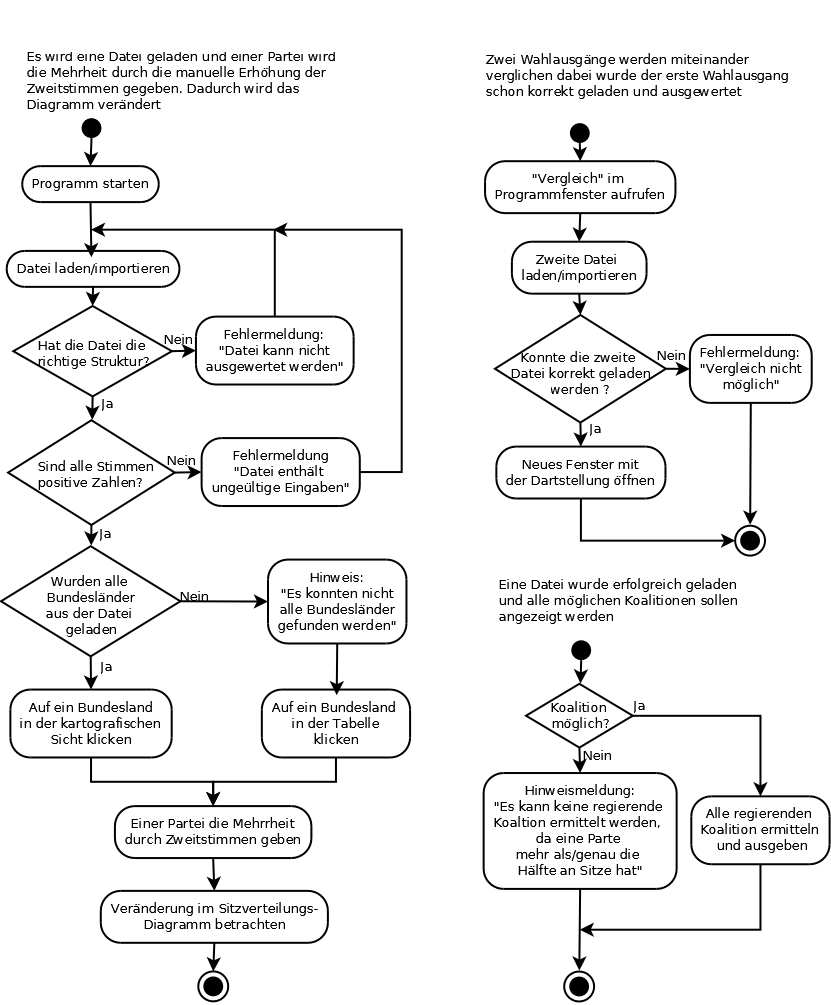
\includegraphics[scale=0.4]{Diagramm3}
\newpage
\subsection{Datenkonsistenzen}
Die folgenden Datenkonsistenzen müssen eingehalten werden:
\begin{itemize}
	\item Die Zustände können nur gespeichert werden, wenn alle geladenen Felder ausgefüllt wurden
\end{itemize}
\subsection{Unzulässige Aktionen}
Die folgende unzulässige Aktionen müssen korrekt behandelt werden:
\begin{itemize}
	\item Keine negativen Werte als Stimmenanzahl
	\item Keine Buchstaben als Stimmenanzahl
	\item Keine Fließkommazahlen als Stimmenanzahl
\end{itemize}
\subsection{Testszenairen}
\subsubsection{Grundlegende Funktionen}
Es werden grundlegende Funktionen des Programms getestet, um sicherzustellen, dass das Programm während der Bearbeitung nicht durch eine fehlerhafte Aktion abstürzt.
\begin{description}
	\item[\textbf{/T0010/}] Zwei Wahlen miteinander vergleichen: \\
	Die Sitzverteilung einer geladenen Datei berechnen $\rightarrow$ Einen neuen Tab öffnen $\rightarrow$ Die neue Importdatei laden $\rightarrow$ Die Sitzverteilung für die neue Wahl berechnen $\rightarrow$ Beide Sitzverteilung miteinander vergleichen
	\item[\textbf{/T0020/}] Manuell einen negativen Wert als Stimmenanzahl eintragen: \\
	Einen negativen Wert als Stimmenanzahl in die Tabelle eintragen $\rightarrow$ Eine Fehlermeldung: ``Negativer Wert'' erhalten $\rightarrow$ Den Wert unverändert lassen
	\item[\textbf{/T0030/}] Manuell einen Buchstaben als Stimmenanzahl eintragen: \\
	Einen Buchstaben als Stimmenanzahl in die Tabelle eintragen $\rightarrow$ Fehlermeldung: ``Buchstaben anstatt einer Zahl eingegeben'' erhalten $\rightarrow$ Wert unverändert lassen \\
	\item[\textbf{/T0040/}] Eine Fließkommazahl als Stimmenanzahl eintragen: \\
	Eine Fließkommazahl als negativen eintragen $\rightarrow$ Fehlermeldung: ``Ganze positive Zahlen anstatt Fließkommazahlen eingeben'' erhalten $\rightarrow$ Wert unverändert lassen \\ 
	\item[\textbf{/T0050/}] Erststimme in der Wahlkreisansicht verändern: \\
	Von der Bundansicht in eine Landansicht wechseln $\rightarrow$ Von der Landesansicht in eine Wahlkreisansicht wechseln $\rightarrow$ Die Erststimmen/Zweitstimmen eine beliebigen Partei verändern $\rightarrow$ Wieder zurück zur Bundansicht wechseln $\rightarrow$ Mögliche Änderung der Sitzverteilung wahrnehmen
	\item[\textbf{/T0060/}] Die Funktion ``Diagramm wechseln'' testen:\\
	Die Sirtzverteilung berechnen $\rightarrow$ Das Diagramm ändern $\rightarrow$ Die Sitzverteilung wird beibehalten
	\item[\textbf{/T0070/}] Die Funktion ``Rückgängig machen'' testen: \\
	Eine beliebige Stimmenanzahl verändern $\rightarrow$ Die Sitzverteilung berechnen lassen$\rightarrow$ Durch ``Rückgängig machen'' den Wert wieder zurücksetzen $\rightarrow$ Die Sitzverteilung wird erneut berechnet
	\item[\textbf{/T0080/}] Die Funktion ```Wiederherstellen'' testen: \\
	Eine beliebige Stimmenanzahl verändern $\rightarrow$ Die Sitzverteilung berechnen lassen $\rightarrow$ Den Wert durch ``Rückgängig machen'' die Aktion zurücksetzen $\rightarrow$ Die Sitzverteilung wird wieder berechnet $\rightarrow$ Durch "Wiederherstellen" den rückgängig gemachten Wert wiederherstellen
\end{description}
\subsubsection{Import-/Exportverhalten}
Die folgenden Testfälle testen das Import-/Exportverhalten des Programms. Dabei wird vorausgesetzt, dass das Programm gestartet wurde und sich im Startzustand befindet. 
\begin{description}
	\item[\textbf{/T0110/}] Struktur einer Importdatei verändern: \newline
	Die Importdatei verändern$\rightarrow$ Im Hauptmenü auf Datei klicken $\rightarrow$ ``Datei importieren'' auswählen $\rightarrow$ Im Dateibrowser die korrupte Importdatei auswählen $\rightarrow$ Mit dem Button ``Laden'' bestätigen $\rightarrow$ Die Fehlermeldung: ``Datei konnte nicht geladen werden'' erhalten
	\item[\textbf{/T0120/}] Zu dem gespeicherten Zustand zurückkehren: \\
	Eine beliebige Importdatei laden $\rightarrow$ Die Sitzverteilung berechnen lassen$\rightarrow$ Den aktuellen Zustand als neue Importdatei speichern$\rightarrow$ Eine beliebige Veränderungen an den Stimmen ausführen $\rightarrow$ Das Programm ohne zu speichern schließen $\rightarrow$ Das Programm wieder öffnen und die Importdatei ohne die Veränderungen laden
	\item[\textbf{/T0130/}] Gleichnamige Parteien in der Importdatei: \newline
	Die Importdatei mit zwei gleichnamigen Parteien laden $\rightarrow$ Fehlermeldung: ``Mehrere Parteien haben den gleichen Namen'' erhalten
	\item[\textbf{/T0140/}] Nur eine Partei befindet sich in der Importdatei: \newline
	Eine beliebige Importdatei mit nur einer Partei laden $\rightarrow$ Sitzverteilung berechnen lassen $\rightarrow$ Fehlermeldung: ``Sitzverteilung mit nur einer Partei nicht möglich'' erhalten
	\item[\textbf{/T0150/}] Importdatei mit fehlerhaften Bundesländernamen: \newline
	Eine Importdatei mit mindestens einem falsch geschriebenen Bundesland laden$\rightarrow$ Fehlermeldung: ``Kartografische Ansicht nicht möglich'' $\rightarrow$ Anstatt der kartografischen Ansicht wird nur die Liste angezeigt $\rightarrow$ Die Sitzverteilung wird weiterhin normal berechnet\newline
	\item[\textbf{/T0160/}] Eigenen Wahlausgang erstellen: \\
	Beliebige Importdatei mit der gewünschten Struktur laden $\rightarrow$ Die Aktion ``zufällige Wahlausgänge generieren'' auswählen $\rightarrow$ Zufällig generierter Wahlausgang unter beliebigen Namen exportieren
\end{description}
\subsubsection{Korrekte Berechnung der Sitzverteilung}
Die folgenden Testfälle testen die korrekte Berechnung der Sitzverteilung. Dabei wird vorausgesetzt, dass  das Programm gestartet wurde und erfolgreich eine Importdatei geladen wurde.
\begin{description}
	\item[\textbf{/T0210/}] Ein Direktmandat fehlt: \newline
	Testweise werden alle Erststimmen eines Wahlkreises gelöscht $\rightarrow$ Die Fehlermeldung: `` Direktmandat fehlt im Wahlkreis'' erhalten
	\item[\textbf{/T0220/}] Mehrere Wahlkandidaten haben gleich viele Stimme in einem Wahlkreis: \newline
	Mehrere Kandidaten haben gleich viele Stimmen $\rightarrow$ Ein Hinweis wird ausgegeben $\rightarrow$ Kandidat wird ausgelost
	\item[\textbf{/T0230/}] Ein negatives Stimmgewicht in einer Wahl provozieren:\newline
	Die Daten so modifizieren, dass ein negatives Stimmgewicht provoziert wird $\rightarrow$ Hinweis: `` Ein negatives Stimmgewicht wurde berechnet'' erhalten
	\item[\textbf{/T0240/}] Partei mit drei Direktmandate und 2.9 Prozent der Zweitstimmen: \newline
	Die Daten werden so modifiziert, dass eine Partei genau drei Direktmandate hat $\rightarrow$ Die Sitzverteilung wird berechnet $\rightarrow$ Die Partei steht danach in der Sitzverteilung
	\item[\textbf{/T0250/}] Überhangmandat testen: \newline
	Die Daten werden so modifiziert, dass eine Partei mehr Direktmandate als durch Zweitstimmen zugeteilte Sitze hat$\rightarrow$ Die Sitzverteilung wird berechnet $\rightarrow$ Ein Hinweis wird ausgegeben: ``Überhangmandat wurde berechnet''
	\item[\textbf{/T0260/}] Ausgleichsmandat testen: \newline
	Die Daten werden so modifiziert, dass eine andere Partei mehr Direktmandate als durch Zweitstimmen zugeteilte Sitze hat $\rightarrow$ Ein Hinweis wird ausgegeben: ``Ausgleichsmandat wurde berechnet''
\end{description}


\section{Systemmodelle}

\subsection{Systemarchitektur}
Das Programm basiert auf der MVC- Architektur, wobei auf eine saubere Trennung der Einheiten Model, View und Controller geachtet wird. Dies sorgt nicht nur für einen flexiblen Programmentwurf, so dass spätere Änderungen bzw. Erweiterungen erleichtert werden, sondern garantiert auch die Trennung kritischer Komponenten, wie der Algorithmusimplementierung, von weniger sensiblen Komponenten, wie der GUI, und dient allgemein der Übersichtlichkeit.

\subsubsection{Modell (model)}
Das Modell ist das Kernstück der Anwendung. Es enthält alle relevanten Daten, beispielsweise die Stimmzahlen, die für die Mandatsverteilung wichtig sind. Sowie die Logik und Algorithmen um das Wahlergebnis zu berechnen.

\subsubsection{Präsentation (view)}
Die Präsentationsschicht bereitet die Daten des Modells auf und stellt sie dem Benutzer als grafische Benutzeroberfläche bereit. Für einige Daten wird es verschiedene Ansichten geben, z.B. eine kartografische Ansicht, eine Diagrammansicht oder eine tabellarische Ansicht.

\subsubsection{Steuerung (controller)}
Zu jeder Präsentation gibt es eine Steuerung, die diese verwaltet und Benutzereingaben und Interaktionen entgegennimmt und entscheidet welche Daten im Modell geändert werden müssen.

\subsection{Systemübersicht}
Bei diesem System wird ein 3-Schichten-Modell verwendet. Die einzelnen Komponenten des Systems lassen sich wie in der folgenden Abbildung auf die einzelnen Schichten aufteilen.
Die GUI Schicht enthält die Präsentationen und Steuerungen des MVC-Architekturmusters, die Interne-Daten und Logik Schicht enthält das MVC-Modell. Externe Daten lassen sich vom Modell aus importieren und exportieren.

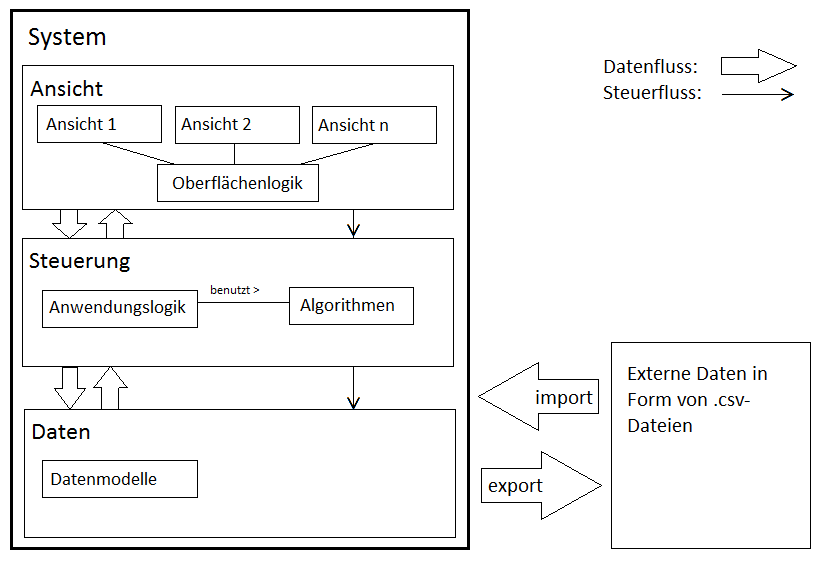
\includegraphics[scale=0.5]{Systemuebersicht2.png}

\section{Benutzungsoberfläche}
\subsection{Bundesansicht}
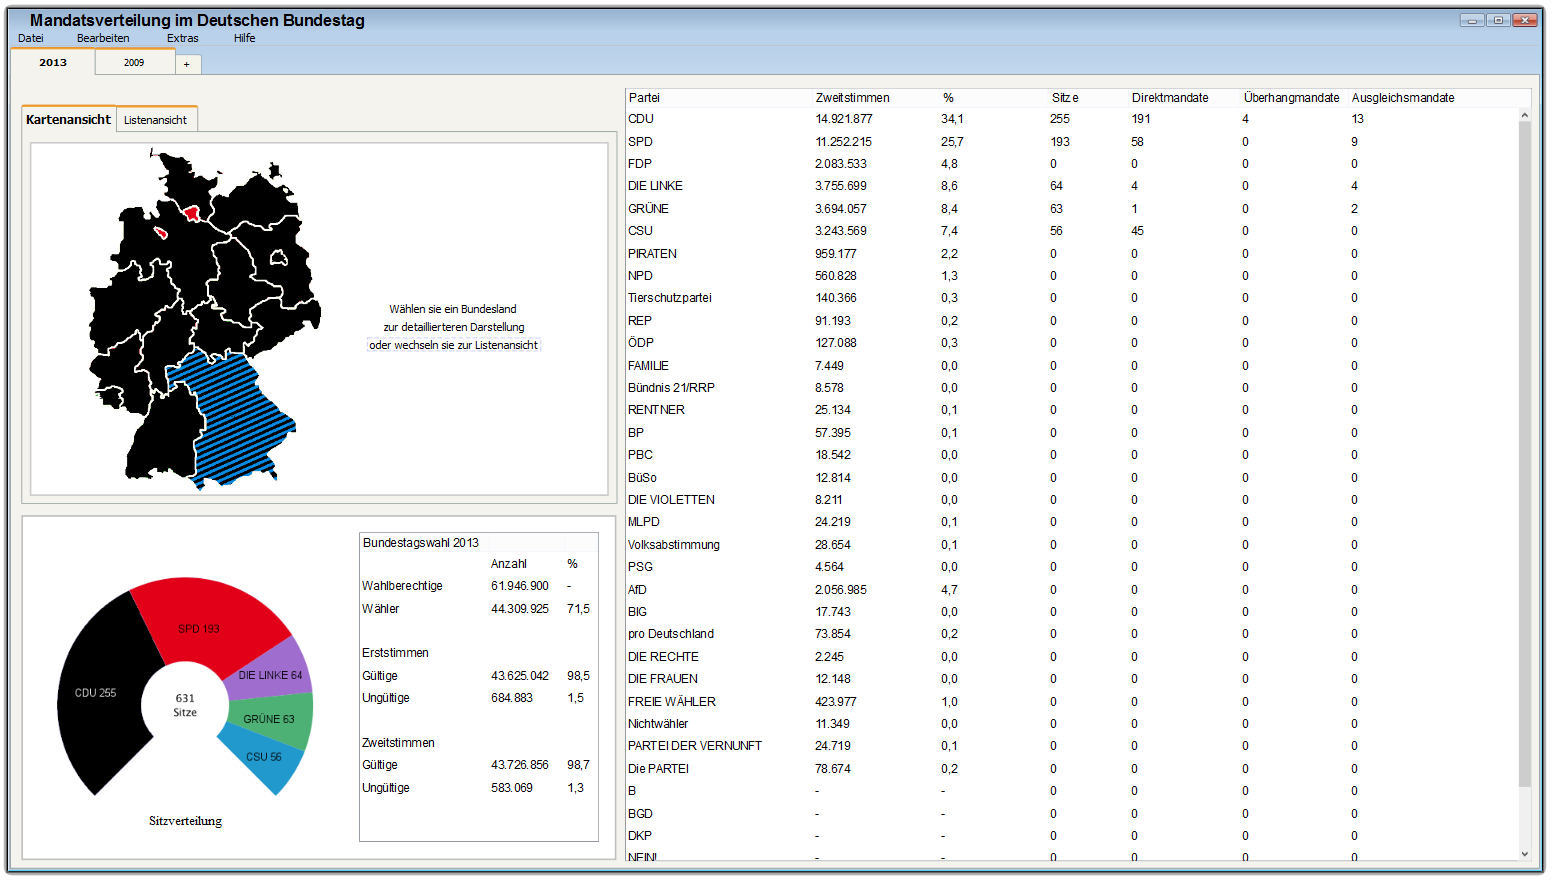
\includegraphics[scale=0.3]{Bundesansicht.png}

\noindent Nach dem Start der Anwendung sieht der Nutzer die Bundesansicht.
In dieser Ansicht sind die Ergebnisse der Bundestagswahl 2013 bereits geladen.
Nach der Auswahl einer Bundeslandes in der Kartenansicht oder der Listenansicht gelangt der Nutzer zur Landesansicht.
\newpage
\subsection{Landesansicht}
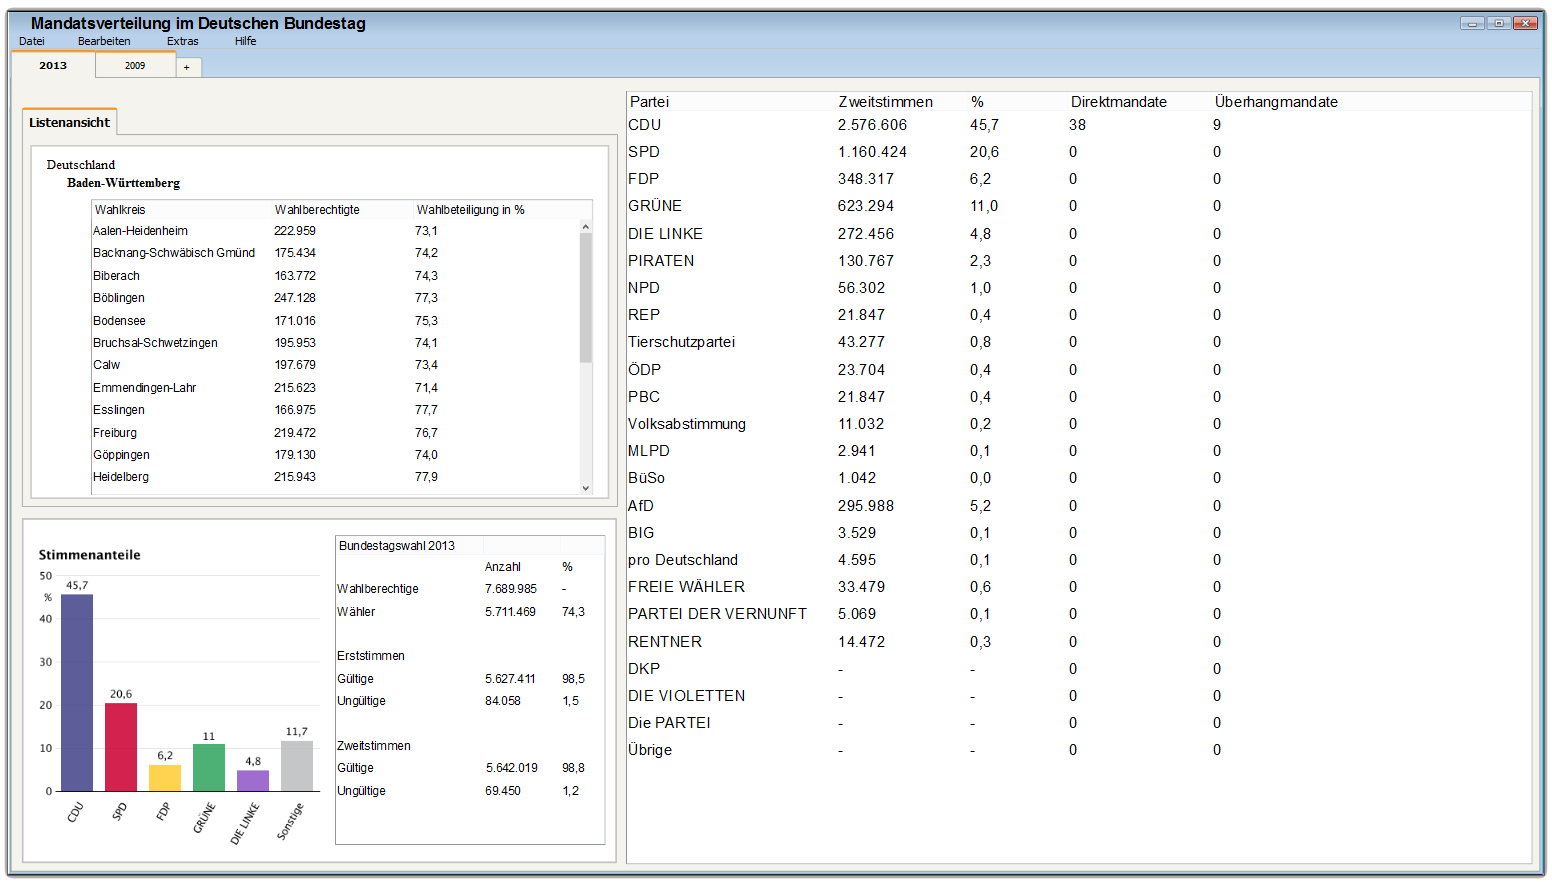
\includegraphics[scale=0.3]{Landesansicht.png}
\noindent In der Landesansicht ist eine Übersicht über die Wahlergebnisse des selektierten Bundeslandes möglich.Durch das Auswählen eines Wahlkreises gelangt der Nutzer zur Wahlkreisansicht.
\newpage
\subsection{Wahlkreisansicht}
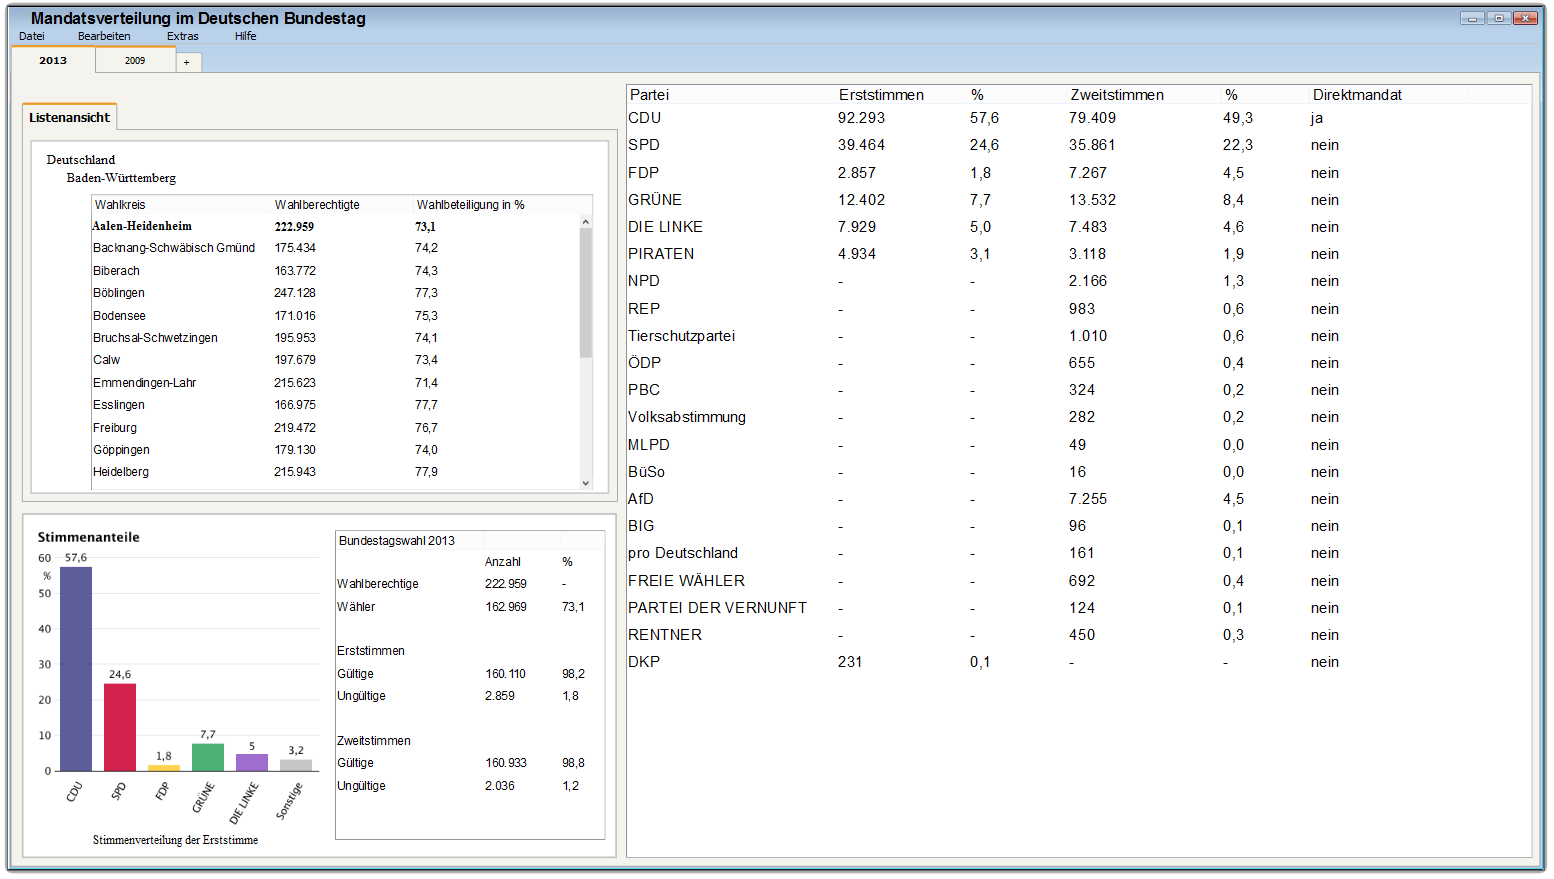
\includegraphics[scale=0.3]{Wahlkreisansicht.png}
\noindent In der Wahlkreisansicht sind die Wahlergebnisse des ausgewählten Wahlkreises übersichtlich dargestellt.
\subsection{Vergleichsansicht}
\includegraphics[scale=0.3]{Vergleichsansicht.png}
\noindent In der Vergleichsansicht kann der Nutzer zwei Wahlausgänge auf beliebiger Ebene (Bundes-, Landes- oder Wahlkreisebene) miteinander vergleichen.
\newpage
\section{Spezielle Anforderungen an die Entwicklungsumgebung}

\subsection{Allgemein}
	\begin{list}{\quad}{}
		\item \textbf{$\LaTeX$} - zur Erstellung von Dokumenten
		\item \textbf{Subversion} (SVN) - zur Versionsverwaltung
		\item \textbf{EtherPad} - zur kollaborativen Bearbeitung von Texten
	\end{list}
	
\subsection{Entwicklung}
	\begin{list}{\quad}{}
		\item \textbf{Eclipse} - integrierte Entwicklungsumgebung (IDE)
		\item \textbf{Swing} - zur Erstellung der grafischen Benutzeroberfläche
	\end{list}
	
\subsection{UML und Diagramme}
	\begin{list}{\quad}{}
		\item \textbf{Pencil Project} - zur Erstellung von GUI-Entwürfen
		\item \textbf{ArgoUML} - zur Erstellung von UML Diagrammen
		\item \textbf{Dia} - zur Erstellung weiterer Diagramme
	\end{list}

\subsection{Qualitätssicherung}
	\begin{list}{\quad}{}
		\item \textbf{JUnit} - zum Testen des Java Quellcodes
		\item \textbf{JaCoCo} (Java Code Coverage Library) - zur Analyse der Testabdeckung
		\item \textbf{Checkstyle} - Code-Analyse zur Prüfung des Programmierstils
	\end{list}

\subsection{Teamkommunikation}
	\begin{list}{\quad}{}
		\item \textbf{Google Groups} - als Mailingliste
		\item \textbf{Google Hangout} - für Sprach- und Videochatkonferenzen
	\end{list}

\section{Zeit- und Ressourcenplanung}

\subsection{Die Phasen des Projekts}
Die zeitliche Aufteilung dieses Softwareprojekts richtet sich nach den fünf Phasen des Wasserfallmodells mit der folgenden zeitlichen Aufteilung und Phasenverantwortlichen.\\
Die einzelnen Phasenverantwortlichen sind dabei dafür zuständig, federführend die ihnen zugeordnete Phase zu organisieren. Außerdem hat der Phasenverantwortliche die Aufgabe in dem Kolloquium am Ende seiner Phase diese in einem kleinen Vortrag vorzustellen und zu berichten was in dieser Zeit getan wurde und wie die Phase verlaufen ist.\\

\begin{tabular}[h]{lll}
	\hline
	\textbf{Phase} & \textbf{Phasendauer} & \textbf{Phasenverantwortlicher} \\
	\hline
	Pflichtenheft & 3 Wochen & Nick Vlasoff \\
	Entwurf & 4 Wochen & Philipp Löwer \\
	Implementierung & 4 (+ 2) Wochen & Anton Mehlmann und Enes Ördek \\
	Validierung & 3 Wochen & Simon Schürg \\
	Interne Abnahme und Abschlusspräsentation & 2 Wochen & Manuel Olk \\
	\hline
\end{tabular}

\subsection{Zeitliche Einteilung der einzelnen Module}
Da dieses Softwareprojekt im Rahmen der Lehrveranstaltungen \textit{Praxis der Softwareentwicklung (PSE)} und \textit{Teamarbeit in der Softwareentwicklung (TSE)} durchgeführt wird, muss sich der Arbeitsaufwand nach den ECTS-Punkten dieser Lehrveranstaltungen richten.\\\\
$PSE + TSE = 6 ECTS + 2 ECTS = 8 ECTS$\\
Ein ECTS-Punkt entspricht üblicherweise 30 Arbeitsstunden $\Rightarrow 8 * 30 Stunden = 240$ Stunden Arbeitsaufwand pro Person. Wir sind insgesamt 6 Personen d.h. es stehen uns $6 * 240 = 1440$ Personenstunden zur Verfügung die Aufgeteilt werden können.\\
Für die Phasen Entwurf und Implementierung planen wir insgesamt 720 Personenstunden ein. Eine genauere Aufteilung dieser Zeit auf die einzelnen Module des dieser Software ist in der folgenden Tabelle dargestellt.\\

\begin{tabular}[h]{lll}
	\hline
	\textbf{Modul} & \textbf{geschätzte Zeit} & \textbf{Verantwortlicher} \\
	\hline
	Import-Export-Modul & 120 Stunden & Enes Ördek\\
	GUI-Design & 160 Stunden & Manuel Olk \\
	GUI-Navigation und Oberflächenlogik & 70 Stunden &  Philipp Löwer\\
	Algorithmen zur Berechnung der Mandatsverteilung & 140 Stunden &  Simon Schürg\\
	Algorithmen zum finden Paradoxer Situationen  & 110 Stunden &  Nick Vlasoff\\
	Diagramme und kartografische Ansicht  & 120 Stunden &  Anton Mehlmann\\
	\hline
	Summe & 720 Stunden & --------- \\
	\hline
\end{tabular}

\subsection{Ressourcen}
Jedes Teammitglied benötigt einen Personal Computer mit Leistungswerten über den Mindestanforderungen für die Entwicklung dieser Software.

\section{Glossar}
\textit{ToDo: glossaries Bibliothek verwenden und Begriffe beschreiben.}
\begin{itemize}
	\item Listenplatz
	\item paradoxe Situationen
	\item Mandat	
	\item Direktmandat	
	\item Überhangmandat
	\item Ausgleichsmandat
\end{itemize}

\end{document}
